% This example An LaTeX document showing how to use the l3proj class to
% write your report. Use pdflatex and bibtex to process the file, creating 
% a PDF file as output (there is no need to use dvips when using pdflatex).

% Modified 


\documentclass{l3proj}
\usepackage{listings}
\usepackage{subcaption}
\usepackage{wrapfig}
% More listing stuff.
%\usepackage{bera}% optional: just to have a nice mono-spaced font
\usepackage{listings}
\usepackage{xcolor}

\colorlet{punct}{red!60!black}
\definecolor{background}{HTML}{EEEEEE}
\definecolor{delim}{RGB}{20,105,176}
\colorlet{numb}{magenta!60!black}
\definecolor{lightgray}{rgb}{.9,.9,.9}
\definecolor{darkgray}{rgb}{.4,.4,.4}
\definecolor{purple}{rgb}{0.65, 0.12, 0.82}
\lstdefinelanguage{JavaScript}{
  keywords={break, case, catch, continue, debugger, default, delete, do, else, false, finally, for, function, if, in, instanceof, new, null, return, switch, this, throw, true, try, typeof, var, void, while, with},
  morecomment=[l]{//},
  morecomment=[s]{/*}{*/},
  morestring=[b]',
  morestring=[b]",
  ndkeywords={class, export, boolean, throw, implements, import, this},
  keywordstyle=\color{blue}\bfseries,
  ndkeywordstyle=\color{darkgray}\bfseries,
  identifierstyle=\color{black},
  commentstyle=\color{purple}\ttfamily,
  stringstyle=\color{red}\ttfamily,
  sensitive=true
}
\lstdefinelanguage{json}{
    %basicstyle=\normalfont\ttfamily,
    numbers=left,
    numberstyle=\scriptsize,
    stepnumber=1,
    numbersep=8pt,
    showstringspaces=false,
    breaklines=true,
    frame=lines,
    backgroundcolor=\color{background},
    literate=
     *{0}{{{\color{numb}0}}}{1}
      {1}{{{\color{numb}1}}}{1}
      {2}{{{\color{numb}2}}}{1}
      {3}{{{\color{numb}3}}}{1}
      {4}{{{\color{numb}4}}}{1}
      {5}{{{\color{numb}5}}}{1}
      {6}{{{\color{numb}6}}}{1}
      {7}{{{\color{numb}7}}}{1}
      {8}{{{\color{numb}8}}}{1}
      {9}{{{\color{numb}9}}}{1}
      {:}{{{\color{punct}{:}}}}{1}
      {,}{{{\color{punct}{,}}}}{1}
      {\{}{{{\color{delim}{\{}}}}{1}
      {\}}{{{\color{delim}{\}}}}}{1}
      {[}{{{\color{delim}{[}}}}{1}
      {]}{{{\color{delim}{]}}}}{1},
}
% Done
\usepackage{hyperref}
\usepackage{amsfonts}
\setlength\parindent{24pt}
\begin{document}
\title{Design and implement your own programming language}
\author{Kyle Simpson\\
		Kristiyan Dimitrov\\
		Darren Findlay\\
		David Creigh\\
		Gerard Docherty}
\date{27 March 2015}
\maketitle
\begin{abstract}

The abstract goes here

\end{abstract}
\educationalconsent
\tableofcontents
%==============================================================================
\chapter{Introduction}
\label{intro}

\section{Project Outline}

For our project we chose project number 3924; design and implement your own programming language. This project involves designing a programming language, by creating a BNF, system diagram, and the syntax and semantics of the language, among others and then implementing it, using a parser, compiler, and abstract machine.

\section{Motivation}

Our Motivation behind the choosing of this particular project is that, especially in the past few years, computing has come to the forefront of teaching. Many parents now want their children to learn how to code to some degree, with computing science now being a much more prevalent subject in primary and secondary schools. Now in our third year of university, we have all taken part in a fair amount of coding, however, none of us have ever attempted to write our own language to code in. This project seemed challenging, but achievable, and very rewarding – not to mention interesting.

\section{Aim}

The aim for this project is to create a graphical programming language that is simple to use and read, and can be picked up by nearly any novice user, but is also powerful, and can be used to create drawings, or edit pictures. Our idea for a simple language came from Processing, a graphical language created by Casey Reas, and the basis for the language is going to be WebGL – a browser version of OpenGL. With this project, we want to create a language that follows what we think are useful and intuitive features in the design of most programming languages, for example using {} for functions and loops and keeping the familiar structure of the for and while loops, and making sure our language follows them, while finding what we believe to be confusing or annoying common features of programming languages, like the double equals for the comparison of two objects, and replace them with what we find suitable and more 

\section{WebGL Background}

Web Graphics Library (WebGL) is a JavaScript API, that makes use of the <canvas> element available in HTML to render interactive 2d/3d graphics. It is a branch of the Open Graphics Library Embedded Systems 2.0 (OpenGL ES 2.0), and is supported by most modern browsers, like Google Chrome and Mozilla Firefox, with no necessary plugin (as it makes use of <canvas>). A WebGL program consists of control code written in JavaScript, and function code (shader code) that is executed by a computer's GPU. 

\section{Outline of report}

The remaining sections of this report will cover the following topics:
\begin{itemize}
	\item Language Tutorial :- This will comprise of a brief introduction to our programming language, which we have named \textbf{Sketch}
	\item Language Reference Manual :- This will contain the grammar, and describe the language
	\item Project Plan :- This will cover a timeline and basic structure of our project, and what we aimed to acheive from it. \textbf{I think so anyway}
	\item Language Evolution :- This will describe the decisions we made for the language syntax and domain, and why we made them.
	\item Compiler Architecture :- This section will cover the 5 different sections of the compiler:
	\begin{itemize}
		\item Lexer and Parser
		\item Code Generator
		\item Shader Manager
		\item Abstract Machine
		\item Module Facade
	\end{itemize}
	\item Development Environment:- The environment(s) that we used to help structure and create this programming language
	\item Test Plan and Test Suites :- An overview on how we tested the language, using what, and any bugs we discovered
	\item Conclusions :- This will cover what, as a team, we learned and discovered during this project, any problems we encountered, and anything we would try differently.
\end{itemize}

%==============================================================================
\chapter{Language Tutorial}
\label{tut}
This chapter comprises of a brief introduction of how to use our language.
\section{Getting Started}
\label{start}
In every language, the first program to write is always 'hello world' - where you would print the words "hello world". However, as this language is mainly a graphical language, the equivalent would be 'hello square', and the aim is to draw a square. In Sketch, the program required to draw a square is:\\
\lstset{%
      basicstyle=\ttfamily\footnotesize\bfseries,
      xleftmargin=.1\textwidth, xrightmargin=.1\textwidth,
      captionpos=b,
      tabsize=4
    }
\begin{lstlisting}[caption={Hello Square},label={lst:tutorial-hello}]
    function init(){
        Polygon square = ({0,0} + {5,0}) * 4;
        draw square;
    }
\end{lstlisting}
To compile any Sketch program, insert the code into the browser page for our project and click "Render". The result of the program will then be shown on the canvas.
\\ [12pt]
Any Sketch program you write will have to consist of at least one function, and variables. These functions and variables can be named anything you like. You can call other functions to help carry out the task, only ones that you have written, as there are no libraries provided in the current version of the language. 
\\ [12pt]
In Sketch, implicit semi-colons exist at the end of every line. This means that, you don't have to end each line with a semi-colon, and whether you do or not will not have an effect on the compilation of the program. 
\\ [12pt]
The draw() function is used to pass the shapes you want to draw to the correct function, so it can be written to the canvas. This will be discussed in detail later.
\\ [12pt]
One way in which you can pass data between functions is by including variables in the calling statement as arguments. However, you can only do this if the function that is being called is expecting the same number and type of variables. An example is:
\begin{lstlisting}[caption={Function Parameters},label={lst:tutorial-parameters}]
    function init(){
        int n = 2;
        function takesParams(int n){
            print(n);
        }
        takesParams(n);
    }
\end{lstlisting}
Here, you see that the calling statement - \textit{takesParams(n);} - provides the correct number and type of arguments. If there was another argument included, for example \textit{takesParams(n, 7)}, or the wrong types, then it would not compile. This will be talked about in more detail in Chapter \ref{func}. As you can see in Listing \ref{lst:tutorial-hello}, the code inside of a function is enclosed by curly braces \{\}. The draw keyword is used to draw any shapes that you have constructed to the canvas. It will take one parameter, either the point,line or polygon that you have constructed. This is a predefined keyword in the language, so you don't have to write it, but you cannot name any of your functions \textit{draw()} as a result. 

\section{Variables and Arithmetic operators}
\label{vars}
This next section will use a more complicated program than before, introducing more features, such as comments, loops, and expand on previously touched on features, such as variables.
\begin{lstlisting}[caption={Comments and Point Addition},label={lst:tutorial-comment}]
#This Program will draw 3 different shapes - triangle, square and pentagon.
//Both of these lines are ignored by the compiler.

function init(){
	int sides;
	sides = 5;
    int counter = 3;
    
    Point pt1 = {3,1}
    pt2 = {1,3}
    
    Line l1 = (pt1 + pt2);
    
    #this will loop for the number of sides
    while(counter <= sides){
        clear;
        Polygon shape =	11 * counter;
        draw shape ;
        counter++;
    }
}
\end{lstlisting}
The initial lines indicate how to show comments in your code in Sketch. Using a hashsign (\#) or a double slash (//) will cause the compiler to ignore all characters until the next newline, and show that the current line is a comment. These can be used to explain how your programs works, and make it easier to read and understand, for you or other users. The 'clear' function in this example is a reserved keyword, and is used to clear the canvas. A reserved keyword is a word that cannot be used otherwise, for variable names, of function calls - 'draw' is one such example we have shown.
\\ [12pt]
As you can see in Listing \ref{lst:tutorial-comment}, there are two ways of declaring variables, explicitly and implicitly. Each variable declaration must include the variable name, which is an alphanumeric string that always begins with a letter. To explicitly define your variable, each variable name must be preceeded by the intended type. For example, the variables 'sides' and 'counter' in Listing \ref{lst:tutorial-comment} are declared explicitly. Explicit declaration allows for the ability to not initialise the variable immediately. Implicit declaration is when the type is not defined by the user, but instead taken from the context. The type is inferred from the initialization of the variable afterwards. For example, 'pt2' in Listing \ref{lst:tutorial-comment} is implicitly defined, and from the context, the compiler will recognise that it is of type Point. However, with implicit types, you must immediately initialise the variable so its type can be inferred.
\\ [12pt]
The while loop in Sketch is of standard format and standard functionality. This means that the condition contained in the parentheses is tested, and if it returns true, then the body of the loop, and whatever statements it may contain, are executed. Then the original condition is retested. if true, it again executes the body. This continues until the condition is false, at which point, the body of the loop is not executed, and the next command outside the loop is executed and the program continues. A while loop has the format: 
\begin{lstlisting}[caption={The "While" Loop},label={lst:tutorial-while},xleftmargin=.35\textwidth,xrightmargin=.5\textwidth,]
while(condition){
	#insert body here
} 
\end{lstlisting}
Sketch has three main types for drawing shapes, lines and so forth. These are Point, Line and Polygon. Lets start with Point; Point is the basis of all possible shapes. Points make the vertices on which the shapes will be drawn about. A point is defined in the following format \{$x$ Coordinate, $y$ Coordinate\}. An example of both implicit and explicit declaration is shown in Listing \ref{lst:tutorial-comment} with 'pt1' and 'pt2'. These points can be added together to create a Line. Lines are a collection of two points joined together. The format for defining a line, shown by 'l1' in Listing \ref{lst:tutorial-comment}, is Line = (Point1 + Point2). Lines can be extended from the centre point by multiplying it by a number. For example, multiplying a line by 4 will make it 4 times the size. Finally, variables of type Polygon are a collection of lines, displayed as a closed circuit. Polygons can be defined by either adding multiple lines together, but they must all join, or by defining one line, and multiplying it by the number of sides you would like. This would create a shape of the stated number of lines, closed off, with the origin being the first co-ordinate of the line. The format of this would be either Polygon = (Line2 + Line2 ... + LineN) or Polygon = Line * N. In these examples, N is the number of sides desired.
\\ [12pt]
The line 'counter++' increments the counter, using the modifying operator '++'. We will explain modifying operators later in this tutorial.
\\ [12pt]
Sketch also has one more type of loop - the "for" loop. The for loop has a completely different structure to the while loop, but has, more or less, the same functionality. The choice between these two types is based on the context, which one would make more sense, for example, incrementations should be used in for loops, while boolean variables should be the control in while loops. The following is the while loop from Listing \ref{lst:tutorial-comment}, changed to a for loop:
\clearpage
\begin{lstlisting}[caption={The "For" Loop},label={lst:tutorial-for},xleftmargin=.1\textwidth,xrightmargin=.1\textwidth,]
    for(int counter = 3; counter < 5; counter ++) {
        ...
    }
\end{lstlisting}

The for loop statement has three parts. Firstly, the control variable is initialised (it also does not need to be declared beforehand), then the statement that will be checked after every execute of the body, and finally, the incrementation of the control variable. The general functionality is the same as the while loop.
\section{If statement and comparitive operators}
\label{comp}
This section will cover how to perform comparing statements in Sketch. The following is an if statement which compares to check if a varaible is equal to something else:
\begin{lstlisting}[caption={If-Else Conditionals},label={lst:tutorial-ifelse}]
    function init(){
        int n = 5;
        if(n ?= 5){
            print(n);
        }
        else if(n ?> 5){
            print("less than 5");
        }
        else if(n ?< 5){
            print("greater than 5");
        }
    }
\end{lstlisting}
If statements are a way of executing a series of commands, but only if a particular statement returns true. To compare to elements, a comparitive operator is needed. In Sketch, there exists a series of six comparative operators:
\begin{itemize}
\item \textbf{?=} will return true if left hand side is equal to right hand side.
\item \textbf{?\textgreater} will return true if left hand side is greater than right hand side.
\item \textbf{?\textless} will return true if left hand side is less than right hand side.
\item \textbf{!=} will return true if left hand side does not equal right hand side.
\item \textbf{!\textgreater} will return true if left hand side is not greater than right hand side (ie is less than or equal to).
\item \textbf{!\textless} will return true if left hand side is not less than right hand side (ie is greater than or equal to).
\end{itemize}
An exclamation mark can be inserted in front of the check statement in the if, to receive the inverse of what it returns.

\section{Modifying Operators}
This section will cover how you can make use of sketch's modifying operators. The following example will outline them:
\begin{lstlisting}[caption={Modifying Operators in Action}, label={lst:tutorial-modify}]
    function init(){
        int n = 1; #line 1
        n += 2; #line 2
        n *= 2; #line 3
        n /= 2; #line 4
        n -= 2; #line 5
        n %= 2; #line 6
        n++; #line 7
        n--; #line 8
        n = (n + 3) * 5; #line 9
    }
\end{lstlisting}
Listing \ref{lst:tutorial-modify} outlines many modifying operators in Sketch. To explain each one, we will walk through the program itself. As previously mentioned, the first line will declare n to be of type int, with a value of 1. The next line will change the value of n by adding one to it. The general syntax would be \textit{*variable to be changed* += *how many to change it by*}. The next three lines follow the same syntax and semantics, with the exception that, line 3 would multiply the variable by the second value and assign it, line 4 would divide it by the second value and assign it, and line 5 would subtract by the second value and assign it, and finally line 6 would change the variable to equal the value of it modulo the second variable. This means that it would change it to the remainder after being divided by that number. So, after line 2, n would be equal to 3, after line 3, n would equal 6, after line 4, n would equal 3, after line 5 n would equal 1 and after line 6, n would still equal 1, as the remainder of 1 / 2 is still 1. These operators are functionally a shorter way of writing \textit{n = n + *value*;}, but obviously changed respective to the context (division, multiplication, subtraction and modulo).
\\ [12pt]
Line 6 is different. This operator will increment the variable by only 1. In the context of this program, n will now equal 2. The following line following the same structure, but instead subtracts one, meaning n is back to equal 1. These can be useful in loops for example, to increment or decrement your controlling variable as necessary. The final line outlines how parenthesis work in regards to performing mathematic actions. The flow it would take, is to first, add  to n, making it equal 4, and then multiply by 5, hence n equals 20. The brackets would specify what task has to be carried out first, as if they were not here on this occasion, by the laws of maths, 3 would be multiplied by 5 and then added to n, giving a different outcome. All of these modifying operators, except on line 9, are functionally just shorthand, but can be very useful and time saving while writing a program.
\section{Functions and Scope}
\label{func}
In Sketch, functions, as mentioned before, taken certain types and number of parameters dependant on what you specify, it can range from 0 to n. Furthermore, these functions can be called whatever you decide, and can either have a return type or not, dependant on your needs. Example 1.6 will show these in action:
\begin{lstlisting}[caption={Functions and Scope}, label={lst:tutorial-functions}]
function init(){
    int x = 1;
    int i = 5;
    function foo(int n) -> int{
        n++;
        return n;
    }
    function foo2(int n){
        n++;
    }
    i = foo(int i);
    foo2(int x);
}
\end{lstlisting}
In Listing \ref{lst:tutorial-functions}, you can see different properties of defining and calling a function. If a function is not returning anything, then you can see that the void is implicit. Furthermore, if a function has a return type, then you can assign a variable to equal its returned value, if it is of the same type. In regards to scope, functions have local scope, meaning that they would alter outside variables, or variables in other functions. This means that, as shown here, you can call variables the same name in two different functions, and there will be no crossover or confusion of values or any conflicts. 


%==============================================================================
\chapter{Language Reference Manual}
\label{manual}

%==============================================================================
\chapter{Project Plan}
\label{plan}

%==============================================================================
\chapter{Language Evolution}
\label{evo}
\section{Graphics programming language or general purpose one?}
The first decision that had to be made regarding the project was what type of language should be developed. The two main types we were considering were graphics programming language or general purpose one.Each of them had its advantages and disadvantages but we decided to go for a graphics programming language since we considered it to be less difficult to implement in theory than a general purpose one. It would be much more interesting for us rather that the other type and we would be able to be create amazing graphs and shapes within just a few lines of code.  

\section {How should our main program look like?}
Our main program consists of 2 functions called init() and render(). Having both of them is not mandatory, but at least one of them should be present into the source file. In init(), the user specifies all variables and expression that he is using. Everything that should be drawn is specified in render(). Of course, the user can use variable declarations and everything else from the syntax, but the draw function should be called from render(). Example can be seen in Listing \ref{main} .

We were considering having only one function called main() for the whole code or not having main function at all, but at the end we decided that having that separation would make our language more readable, easy to learn and initiative for every user.
\begin{center}
\lstset{
    basicstyle=\small\ttfamily,
    frame=lrtb,
  }
 

 
  \begin{lstlisting}[caption= {Main program in Sketch}, label= {main}]
  function init(){
    //variable declarations
  }
 
  function render(){
  // draw()
  }
  \end{lstlisting}
  \end{center}
 
\section{What should be the primitive  types in our language?}
The initial selection of primitive types consisted of \textbf{int, float, double, vector, Point} and \textbf{String}. We thought that these 6 types would be enough for our language.We were considering having a single \textbf{num} type, which we replace all the numerical types, but this idea was quickly rejected, since we reckoned that it would limit the functionality of Sketch and would cause a lot of ambiguities in given circumstances.

Prior to the beginning  of the implementation, we made a new change in our primitive types. New type \textbf{bool} was added to the initial set, because we decide that it would be useful in situations where the validity of given condition should be met. Instead of having float and double, we agreed on one type \textbf{float}, which would combine these two, since  they were increasing the complexity of our language.  


At the end, two new types were added \textbf{Line} and \textbf{Polygon} as we assumed that they would be necessary for the special kind of arithmetic that the language can perform. The final list of primitive type of Sketch is \textbf{bool, int, float,vector, String, Point, Line and  Polygon}.

\section {Function declaration}
After some considerations, it was decided that function will be declared using \textbf{function} keyword followed by its name and list of parameters. The challenging bit here was how to specify the return type. The two options were either having it at the beginning of the declaration as in some programming languages or just after the parameters list specified by "-\textgreater" and the return type (similar notation is used in Swift programming language). We decided to go for the second one, because using  "-\textgreater" is similar to what is used in mathematical functions for mapping one domain to another and this would be appropriate for the context of our programming language.

Another feature, that is inspired for Swift, is the implicit void of a function. If a return type is not specified, then the function is void. This would increase the flexibility and usability of our language.
A possibility for multiple return types was consider, but we decided at this initial stage it would increase the complexity and it would possibly be a reason for confusion of our users.

\section{Comparison operators}
Very often it is confusion for inexperienced programmers to distinguish between assignment operator( often '=') and comparison operator for equality(often "=="). We decided to introduce a completely different notation for comparison. In order to check if two variables are equal, we use \textbf{"?="}. For consistency reasons, operators for less than and greater are \textbf{'?\textless'} and \textbf{'?\textgreater'}. We believe that this makes Sketch easier for new programmers and it makes is unique since we haven not seen these kind of notation in any other language.
\section {Semicolons}
Semicolons are very often a reason for compilation errors, but meanwhile it makes the code more readable. In order to limit the possibility of errors, semicolons in our language are optional.
\section {Loops}
We were considering the idea of having only one type of iterator in Sketch, but having in mind that some users prefer 'for-loop'-s,other 'while-loop'-s, we decided our syntax to have all of the most common loops. Having only one iteration statement would limit the flexibility of our language and some of our users would not be happy with this.
 
\section {If statements and switches }
Sketch has if statements and supports if-else as well. We wanted to have switches in our language, but due to time constraints, we decided to keep this structure for later versions of our language.

\section{Other parts of the syntax}
For parts of the syntax not mentioned above, quick decision was made. We wanted our language to be easy to learn by everyone so having syntax not consistent with other programming languages would change this (especially for experienced programmers). Sketch's syntax is similar to the syntax of two of leading programming languages Java and C. 



%==============================================================================
\chapter{Compiler Architecture}
\label{arch}

%------------------------------------------------------------------------------
\section{Overview}
\label{arch-over}

Our program module, as part of the role it plays, contains a combination of a compiler, bytecode executor and WebGL interface - written in JavaScript as required by the platform. This section aims to provide a view of the overall architecture and connection between these components, as well a brief explanation of each component's function and design considerations.

The core language module can be divided into 5 main parts:
\begin{enumerate}
\item \textbf{Lexer and Parser} --- The program component charged with tokenising and interpreting Sketch programs, generating an abstract syntax tree for use in code generation.
\item \textbf{Code Generator} --- The program component responsible for conversion of abstract syntax trees into bytecode sequences, for execution by the abstract machine.
\item \textbf{Shader Manager} --- An active subsystem of the module responsible for management, selection and execution of shader programs for drawing at runtime.
\item \textbf{Abstract Machine} --- The main active subsystem present in the module, responsible for all runtime code execution. The abstract machine relies on the shader manager to make draw calls, but handles direct WebGL manipulation for certain key functions separately.
\item \textbf{Module Facade} --- The active component responsible for managing the interconnections and operation of the above components, as well as exposing the module interface to programmers.
\end{enumerate}
Individual and detailed discussion of each system is provided below. The module's subsystems are then connected as shown in Figure \ref{fig:sketch-overall}.
\begin{figure}[!h]
\centering
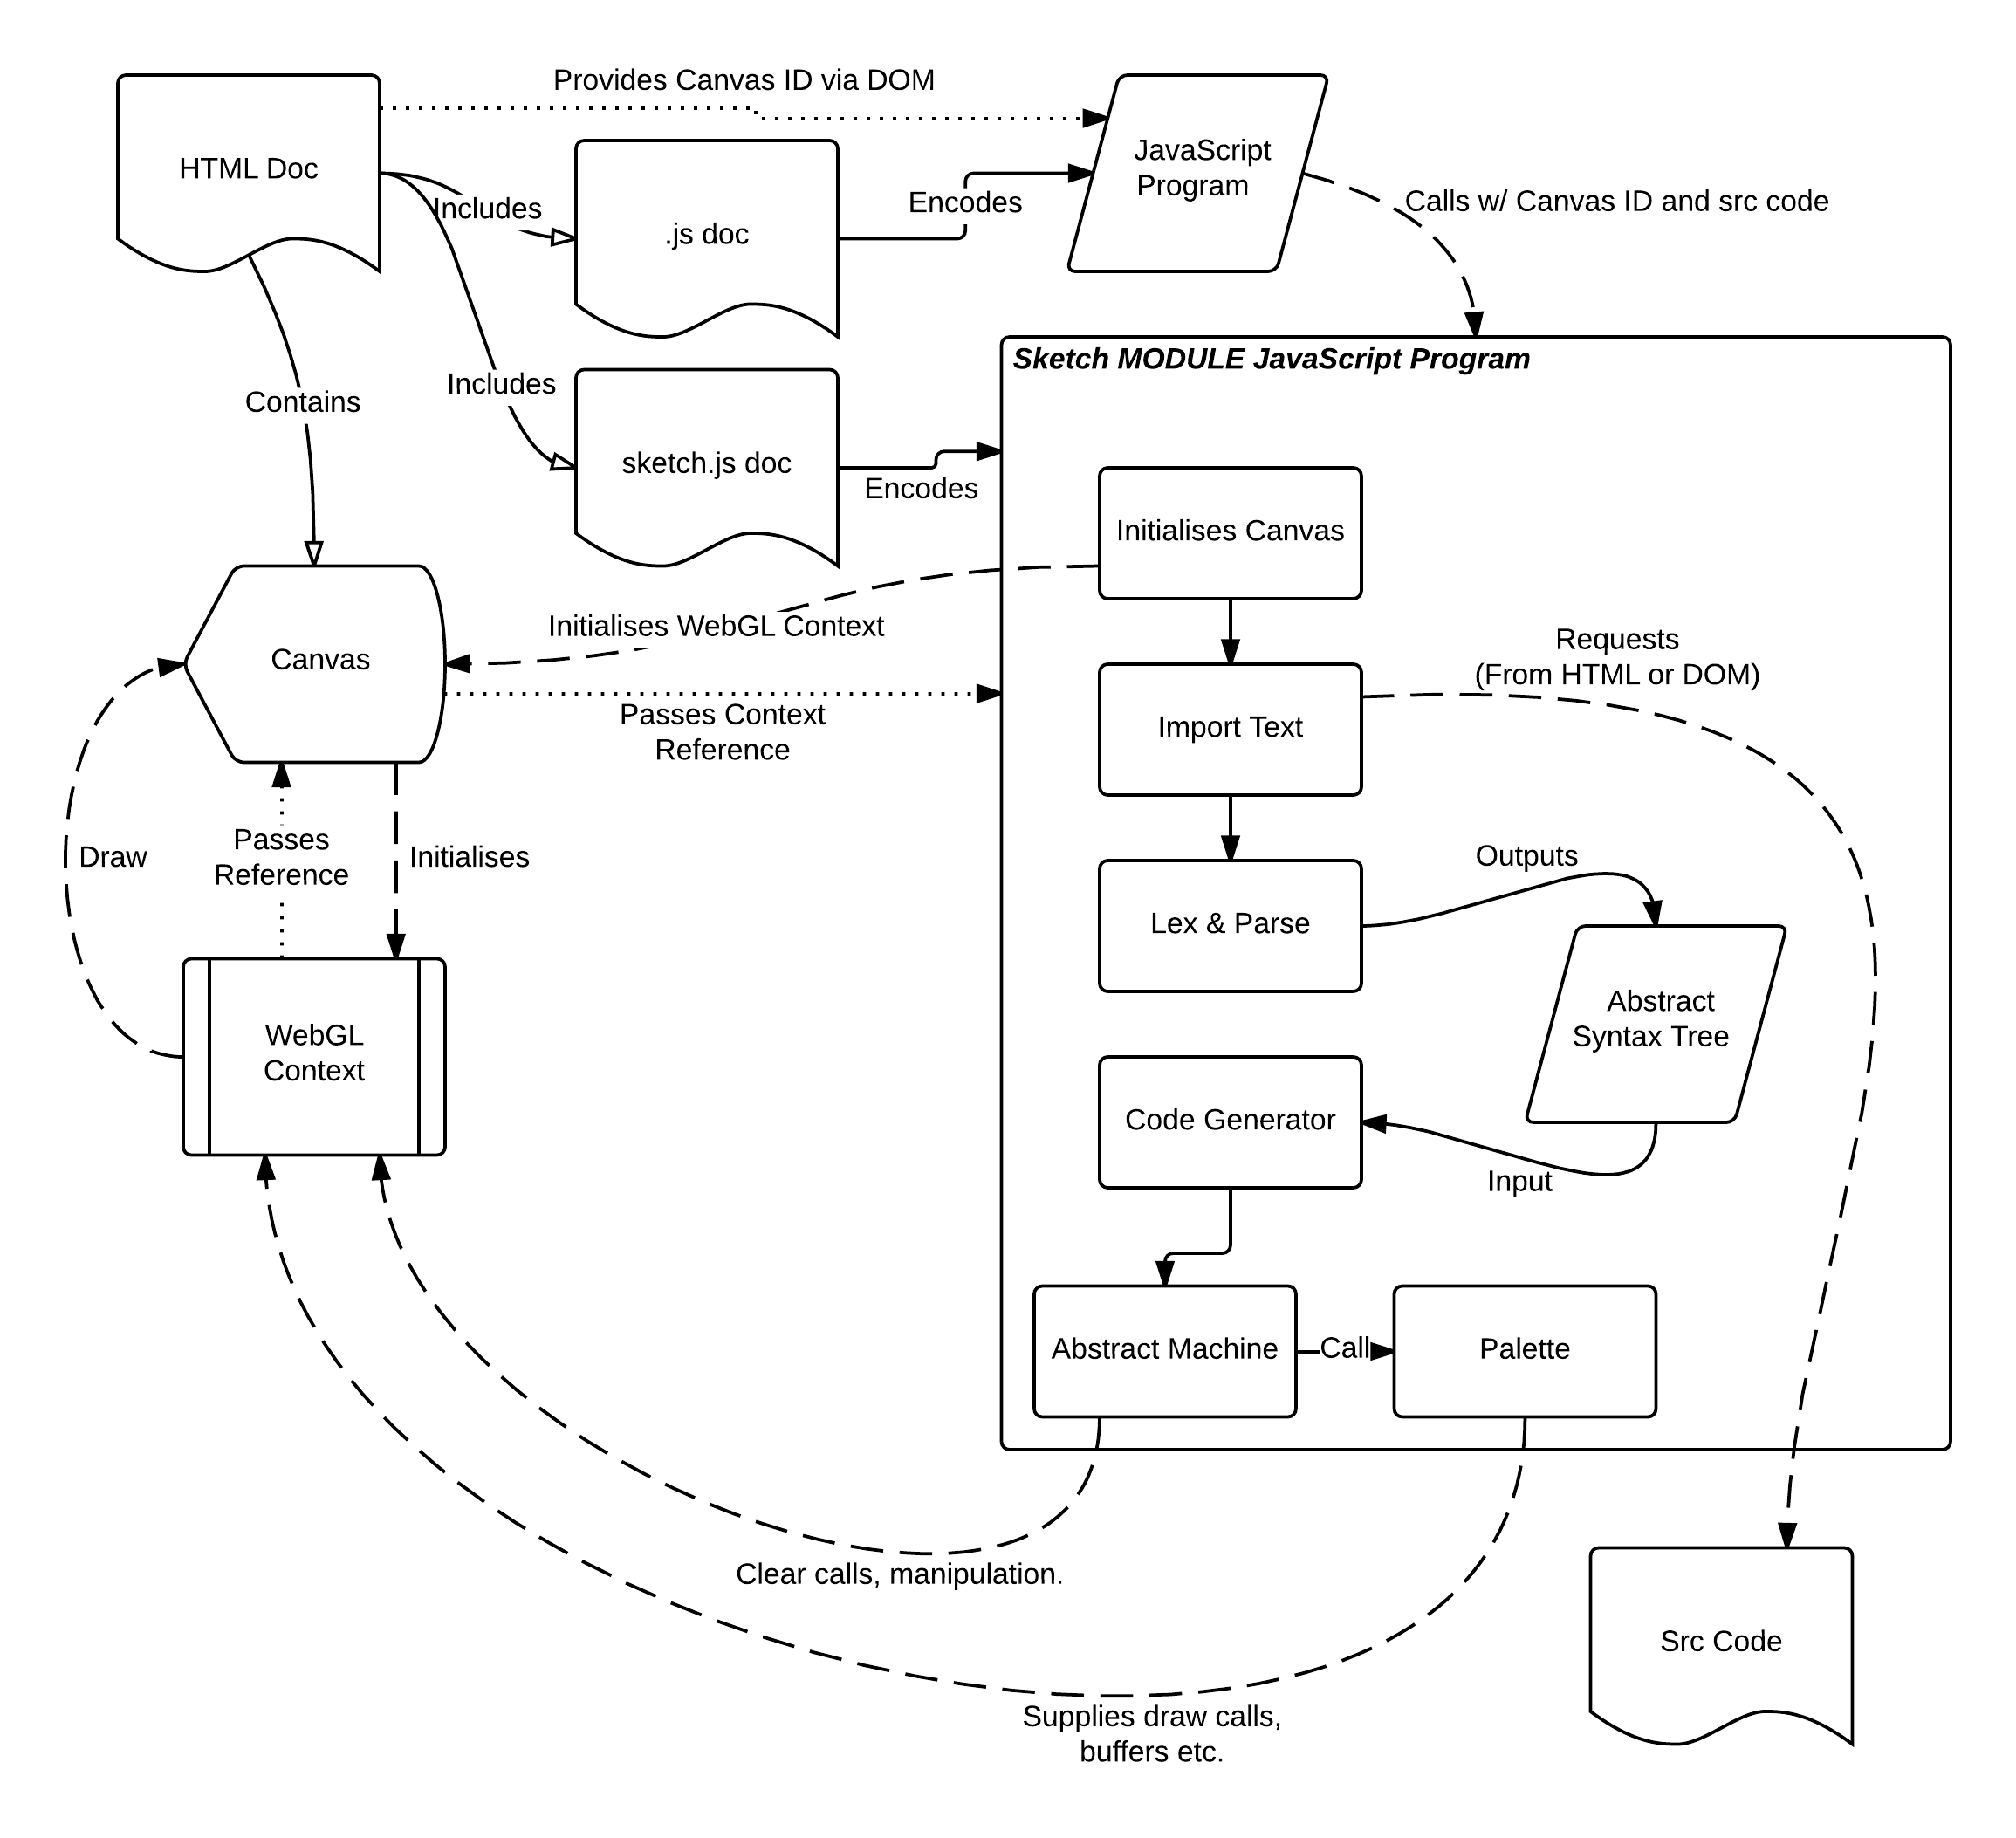
\includegraphics[width=\textwidth]{images/sys-diag}
\caption{Overall system diagram of Sketch, including data flow and interactions with the browser.}
\label{fig:sketch-overall}
\end{figure}

%------------------------------------------------------------------------------
\section{Lexer and Parser}
\label{arch-lex}
\subsection{Introduction}
The lexer and the parser are both part of the syntactic analysis of the compiler. During this stage, a source program is parsed in order to determine if it is well-formed, and to determine its phrase structure , in accordance with the syntax of our programming language. If the source program complies with the syntax and grammar of Sketch, an abstract syntax tree(AST) will be returned from the parser. An AST is a way to represent a source program’s phrase structure. 

\subsection{Initial steps}
At the beginning of implementing parser and lexer for our grammar, an appropriate parser generator for JavaScript had to be found. We found three possible parser generators, each of which would helped us with desired result. ANTLR, JISON and PEG.js were considered as possibilities.
\\[12pt]
ANTLR uses LL(*) parsing and it can generate lexers,parsers, tree parsers and lexer-parsers. Parsers produced by it are able to automatically generate an AST, which was necessary for our design. However, the most recent release of the software (ANTLR 4) does not support JavaScript as a target source, even though the previous version does. 
\\[12pt]
JISON and PEG.js do not encounter the same program - they successfully support JavaScript as a target and both could have been appropriate choice for our parser. PEG.js is based on parsing expression grammar formalism, which is more powerful that traditional LL(k) and LR(k) parsers. On the other hand, Jison can recognize languages described by LALR(1) grammars and provides additional features(i.e the ability to define operator associations and precendence). Because of this additional features, JISON was our choice for parser generator. 


\setcounter{secnumdepth}{3}
\subsection{Design}
JISON provided us with the opportunity to specify both tokenizing rules and language grammar in the same file. This turn out to be very helpful in latter stages when the communication between the parser and code generator had to happen. The whole design process is comprised of three stages: lexical analysis, specification of the grammar and specification of the abstract syntax tree in JSON format. 

\subsubsection{Lexer}
Lexer is a program or function that performs lexical analysis (the process of converting a sequence of characters into a sequence of tokens).
A token consist of a token name and attribute value. The token name represents a kind of lexical unit(i.e. keyword,identifier) and later the token names are processed by the parser. 

For each keyword of  our language, a token was specified in the grammar file. Each of the operators and punctuations symbols have a specified token as well. There are tokens for the identifiers, numbers and strings as well. This way, all the possible tokens for Sketch were covered in the grammar file. In Listing \ref{lst:token-example}, an example for each of them is presented. 
\begin{center}
\lstset{
    basicstyle=\small\ttfamily,
    frame=lrtb,
  }
  

  
  \begin{lstlisting}[caption={Tokens of Sketch },label={lst:token-example}]
  %lex
  %% 
  ...
  "if"                      return 'IF';
  "Line"                    return 'LINE';
  ...
  "{"                       return 'OPEN_BRACE';
  ...
  "+"                       return 'PLUS';
  ... 
  [0-9]+("."[0-9]*)?        return 'NUMBER';
  [a-zA-Z_]+[a-zA-Z0-9_]*   return 'IDENTIFIER';
  /lex
  \end{lstlisting}
\end{center}

\subsubsection{Grammar}
Next stage in the implementation for this part of the compiler was to specify the grammar rules for our graphic programming language. All the rules specified in the initial BNF were translated in a format that the parser generator can accept. 

As a result, in the case when a given rule of the grammar can be used, that rule had to be rewritten again  but this time using the recursion feature of JISON. JISON supports 2 types of recursion - left and right, but our grammar uses left recursion, since it more reliable and it can parse a sequence of any number of elements with bounded stack space.


Another feature of JISON became very useful in the elimination of shift-reduce conflicts - the ability to specify precedence. Initially our grammar was full of shift-reduce conflict because of the \textit{"dangling else"}  in \textit{"condtion\_statment"} (Listing \ref{lst:shift-example}). By using precedence, our grammar become less ambiguous and errors are less likely to occur. 

\begin{center}
\lstset{
    basicstyle=\small\ttfamily,
    frame=lrtb,
  }
  

  
  \begin{lstlisting}[caption={condtion\_statments in Sketch after removal of Shift-Reduce conflict },label={lst:shift-example}]
condition_statements
: IF OPEN_PARENS exp CLOSE_PARENS statement
									 %prec IF_WITHOUT_ELSE
    ...
| IF OPEN_PARENS exp CLOSE_PARENS statement ELSE statement
    ...
;
  
  \end{lstlisting}
\end{center}

\subsubsection { Abstract Syntax Tree (AST)}
If a source program in Sketch uses the correct syntax and grammar rules, after parsing an Abstract Syntax Tree would be generated and passed to the code generator. Our parser produces a tree represented as an object in JSON format. As a result, the JISON file had to be changed and for each grammar rule the corresponding JSON object was added. In Listing  \ref{lst:ast-example}, the output for \textbf{"Hello Square"} program is show.
If one of the grammar rules is violated, no AST will be generated and error will be thrown - this feature is provided for us by the parser generator.

\lstset{%
      basicstyle=\ttfamily\footnotesize\bfseries,
      frame=single,
      xleftmargin=.1\textwidth, xrightmargin=.1\textwidth,
      captionpos=b,
      tabsize=4,
      language=json
    }
\begin{lstlisting}[caption={Sample AST produced by the parser },label={lst:ast-example}]
{
 "type":"function",
  "arguments":
      ["init","","void",
         [{"type":"variable-decl-assign",
            "arguments":
             [["Polygon","square"],
                 {"type":"multiplication",
                   "arguments":
                     [{"type":"addition",
                        "arguments":[["0","0"],["5","0"]]}, "4"
                     ]
                  }]},
             ["draw","square"]
             ]
            ]
}

\end{lstlisting}
%------------------------------------------------------------------------------
\section{Code Generator}
\label{arch-gen}

%------------------------------------------------------------------------------
\section{Virtual Machine}
\label{arch-abs}

\subsection{Introduction}
The Sketch Virtual Machine is an abstract computing machine. It bridges the gap from the Sketch programming language to javascript and the WebGL API and provides an intermediate language stage for compilation. The instruction set provided by the Sketch Virtual Machine is tailored specifically to implement the operations of the Sketch programming language.

As Sketch is a programming language for drawing graphics on webpages, the Sketch Virtual Machine must be able to run in a browser environment. As Javascript is supported by most modern browsers and is the implementation language for WebGL, it was decided that the Sketch Virtual Machine would be implemented using javascript. This makes Sketch a very portable programming language as it can be run on any machine that can run a browser with Javascript support.

Talk a bit about the Sketch Virtual Machine knowing nothing of the sketch programming language, or how some instructions are tightly coupled with the sketch language.
Talk a bit about how the Sketch Virtual Machine is tightly coupled with the shader management system for drawing.

\subsection{Structure of the Sketch Virtual Machine}

\subsubsection{Data Types}
The Sketch Virtual Machine operates on two kinds of types: Primitive types and reference types. These types can be operated upon, stored as variables, passed as arguments into functions and returned by functions. 

The Sketch Virtual Machine assumes type checking is done at the compilation stage and does no type checking at runtime. Instead, the Sketch Virtual Machine determines its operand types from the instructions. For example, IADD (Integer add), FADD (Float add) and PTADD (Point add) infer that their operands are integer types, float types and point reference types respectively. 

\subsubsection{Primitive types}
The Sketch Virtual Machine supports a three primitive types: \textit{Integer}, \textit{Float} and \textit{Boolean}.
\begin{itemize}
	\item \textit{Integer:} Represents 53-bit signed integer values. Has a default value of 0. 
	\item \textit{Float:} Represents 64-bit signed integer values. Has a default value of 0.
	\item \textit{Boolean:} Represents the logical values true and false. Has a default value of false.
\end{itemize}
All primitive data types in the defined by the Sketch Virtual Machine are stored in 64-bits. This is due to javascript using a single 64-bit type: Number, to represent all numeric values.
Boolean values are actually Integer types. Zero represents false and any non-zero value represents true.

\subsubsection{Reference Types}
Structs in the sketch programming language are represented as arrays. Each struct member is mapped to an index of the array. These arrays exist in the Constant Pool data structure produced by the compiler. Instructions that operate on structs, such as PTADD, have operands that are addresses into the Constant Pool. These address are Integer values.

\subsubsection{Run-time Data Areas}
The Sketch Virtual Machine has four special purpose Registers: Program Counter, Code Limit, Stack Pointer and Frame pointer.
\begin{itemize}
	\item\textit{Program Counter:} The program counter holds the address of the next instruction to be executed in the code store.
	\item\textit{Code Limit:} The code limit holds the address in the code store that comes immediately after the last instruction.
	\item\textit{Stack Pointer} The Stack pointer holds the address of the location immediately above the topmost element on the stack.
	\item\textit{Frame Pointer} The Frame Pointer holds the address of the first element in the topmost frame on the stack.
\end{itemize}
%------------------------------------------------------------------------------
\section{Shader Manager}
\label{arch-shad}

\subsection{Introduction}
\label{arch-shad-intro}
In designing our system, we established that regardless of the chosen compilation and execution pathway all of our library's shaders would have to be intelligently managed; both during runtime and for storage purposes inside the module itself. While an extensive system like Palette may seem too broad in scope for Sketch's module in its current form, at the language's inception we wanted custom shapes and shaders to be a defining feature of our platform. As such, Palette allows us to one day realise our initial ambitious vision of Sketch due to the level of extensibility and portability it provides.

\begin{figure}[!h]
\centering
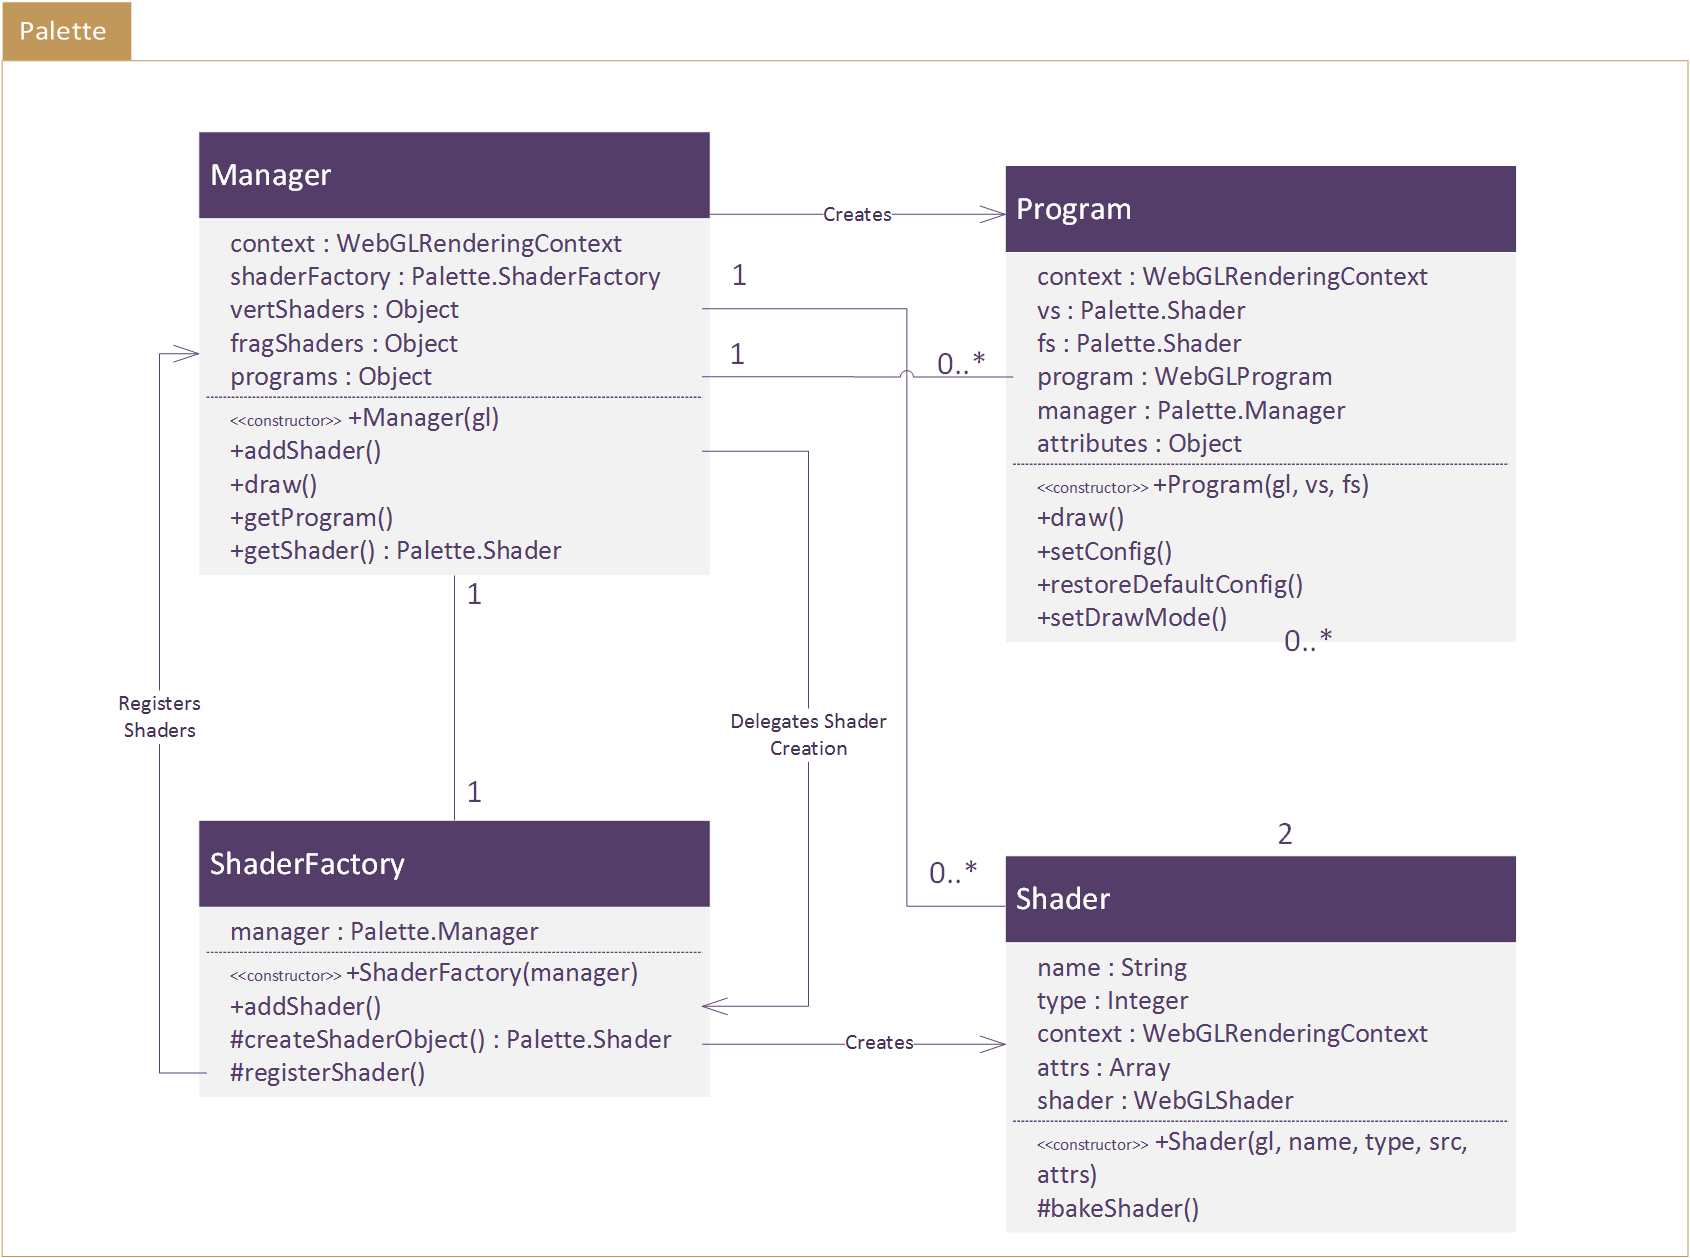
\includegraphics[width=\textwidth]{images/Palette-UML}
\caption{A UML class diagram of Palette.}
\label{fig:palette-uml}
\end{figure}

\subsection{Definitions}
\label{arch-shad-def}
\textit{Shaders} are the graphics card level program units used in the conversion from vertex arrays into two-dimensional projections in the screen space, and in the selection of pixel colours to populate the screen space from that projection. In WebGL, older versions of OpenGL and in its subsets such as GLES, shaders must always come in pairs: a \textit{vertex shader} and \textit{fragment shader} comprise each \textit{shader program}. This may then be accessed, modified and called through the \textit{WebGL API}.


\subsection{Requirements}
\label{arch-shad-req}
The unique needs of our module created an interesting set of design requirements for the subsystem - mandating a somewhat in-depth understanding of the WebGL API to manipulate the canvas as required. Upon examination, the shader manager's requirements were found to be:
\begin{itemize}
\item \textbf{Extensibility} --- Sketch needed to support future extension with various shapes, shaders and other such additions beyond its standard library - most shader programs require writing specially tailored code in an object's .draw() method. Similarly, modifications to shader code often require changes at the software level if the attributes or buffers must be changed - this coupling must be minimised or eliminated.
\item \textbf{Portability} --- Such tailored draw code cannot be imported without putting users at significant security risk by requiring them to execute arbitrary code. Some way to infer the attribute update process from the shader itself is a necessity.
\item \textbf{Ease of Use} --- Definition of new shader files should be intuitive and an easy process, provided the user has valid shader code. The linking and compilation of shaders and shader programs must be handled internally, and completely sequestered from external control to centralise most of the API manipulation.
\item \textbf{Configurability} --- Shader programs should have variable control methods exposed as an external interface, to provide a simple means of control over the intricacies of the WebGL API. For instance, programmers must be able to change the draw mode on a moment's notice, or even extract the shader program pointer if they require direct access to WebGL.
\item \textbf{Simplicity} --- Interactions with the module should be designed with brevity in mind - being able to execute variable update and draw functions as a single method call makes WebGL usage simpler in the other subsystem implementations - lowering the barrier of entry. WebGL is plagued by esoteric function names, inconsistent function prototypes and an arcane set of named constants: all of which must be used regularly to render graphics.
\end{itemize}

\subsection{Design Process and Issues}
\label{arch-shad-design}
The first challenge encountered stemmed from trying to find a way to pass shape definitions within our language. At first, we reasoned that since shapes and objects traditionally have predefined draw functions then we'd need to find a way to export raw JavaScript for each shape class. As mentioned in the requirements, we found that direct code evaluation would not only require difficult scoping considerations but would also present a massive security risk to users of the system. From here, we considered merely assigning shape classes a pair of shaders - this seemed to be the logical choice.

We had originally considered allowing programmers to add shader object JSON from a URL source; this would provide an even more convenient set-up for the manager by reducing shader registration to a single line of code per file. However, we ran into trouble with the management of asynchronous execution calls caused by the main thread running while the download completed. We briefly considered making the HTTP request synchronous, but this caused the entire window to freeze until downloading had completed - we quickly discarded this plan for the time being.

Although our JSON system of "[name, type, default]" worked well for numeric and matrix attributes, we were originally at a loss for how buffers and vertex attributes should be handled. By forcing programmers to supply a buffer object with a known name as well as a vertex attribute specific to their shader code, we managed to bypass this problem with regards to the vertex buffer. We found that using the default value to store the name of the referenced buffer was an eloquent solution - keeping each array to size 3. As far as buffers were concerned, we then realised that we could perform the same substitution to store the itemSize of a buffer. There are many other possible configuration options which had to be cast aside (stride, offset, etc.) to allow this simplicity, however.

Midway through the development of the abstract machine, we realised that we needed a means to convert from planar polygons (like those that Sketch works with) into triangle sets to render any geometry to the screen. While researching polygon triangulation algorithms we came across \textit{earcut} (https://github.com/mapbox/earcut), a JavaScript library which provides the features and speed that our platform would need to make use of. By patching in an extra draw mode to Palette on top of the standard WebGL modes, the simplicity of execution at the abstract machine level was maintained.

While discussion of the implementation details themselves would be appropriate in a dedicated paper, they must unfortunately be omitted as they are outside of this report's scope.

\subsection{Usage}
\label{arch-shad-use}

While JSDoc automatically generates the API documentation for Palette, construction of Shader JSON files is not yet documented. As these are an essential part of Sketch's operation, and shader source code will not suffice on its own, a light explanation is provided.

Shader JSON objects may fall into three types:
\begin{enumerate}
\item \textbf{Vertex Shaders} --- Objects following the form of Listing \ref{lst:vtx-shad-example}, with type set to 0 and at least two attributes: a \textit{buffer} named "vertexBuffer" with default value set to the number of components per vertex, and a \textit{vertexAttrib} with a name matching an attribute within the shader and default value set to "vertexBuffer". Further attributes are defined in the same format as fragment shaders.
\item \textbf{Fragment Shaders} --- Objects defined similarly to Listing \ref{lst:frag-shad-example}, with type set to 1 and no restriction on what attributes must be predefined.
\item \textbf{Shader Lists} --- Objects following the structure of Listing \ref{lst:list-shad-example}, with type set to 2 and the content tag corresponding to an array of further shader objects of any type.
\end{enumerate}
All integer and vector types are supported, along with their array equivalents. These are denoted as \textit{int}, \textit{int[]}, \textit{float}, \textit{float[]} with vectors taking the form \textit{ivec$n$}, \textit{ivec$n$[]}, \textit{vec$n$} and \textit{vec$n$[]} for $ n \in [2,4]\cap\mathbb{N}$. Float matrices may be defined by \textit{mat$n$}, for $n$ within the same domain.
\begin{center}
\lstset{%
      basicstyle=\ttfamily\footnotesize\bfseries,
      frame=single,
      xleftmargin=.05\textwidth, xrightmargin=.05\textwidth,
      captionpos=b,
      tabsize=4,
      language=json
    }
\begin{lstlisting}[caption={Vertex Shader JSON Structure},label={lst:vtx-shad-example}]
{
	"type": 0,
	"name": "squareVtx",
	"src": "#version 100; attribute vec3 aVertexAttrib;//...",
	"attrs": [
		["aVertexAttrib",
		"vertexAttrib",
		"vertexBuffer"],
		
		["vertexBuffer",
		"buffer",
		3]
	]
}
\end{lstlisting}
\begin{lstlisting}[caption={Fragment Shader JSON Structure},label={lst:frag-shad-example}]
{
	"type": 1,
	"name": "squareFrag",
	"src": "//source",
	"attrs": [
		["name",
		"type",
		"default"]
	]
}
\end{lstlisting}
\begin{lstlisting}[caption={Shader List JSON Structure},label={lst:list-shad-example}]
{
	"type": 2,
	"content": [
		{
			"type": 0,
			"name": "...",
			"src": "...",
			"attrs": [...]
		},
		{
			"type": 1,
			"name": "...",
			"src": "...",
			"attrs": [...]
		}
	]
}
\end{lstlisting}
\end{center}
Initialisation of Palette as part of a JavaScript program is a very simple process. Once the module has been included in the execution space through either loading by the browser over HTTP or concatenation as part of a build script, the API is accessible. An example integration is as follows:
\begin{lstlisting}[caption={Palette Usage Example},label={lst:palette-example},language=JavaScript]
//Given a <canvas> element with id "myCanvas".
//The shader text has been imported either by XMLHttpRequest
//Or has been embedded as a string literal into variable 'text'

//Retrieve elements from DOM, and the context from the canvas.
var canvas = document.getElementById("myCanvas");
var glctx = canvas.getContext("webgl");

//Create and set up Palette.
var manager = new Palette.Manager(glctx);
manager.addShader(text);

//Now we're ready to draw!
manager.draw("vsName", "fsName", [/*DATA*/],
			{/*vsConfig*/}, {/*fsConfig*/});
\end{lstlisting}

The full API documentation is available under docs/index.html within our repository (and the deliverables folder supplied) under the namespace "Palette".

\subsection{Future Changes and Evaluation}
\label{arch-shad-future}
While Palette provides a sizeable kernel of features, there is still much room to improve the module - not only to supply all of the functionality we'd originally planned, but also to enable its use in external projects of all scopes.
\begin{itemize}
\item \textbf{Texture Support} --- an absolute necessity to enable images and texturing within Sketch, and for almost all conceivable WebGL projects. Textures require vast amounts of configuration - the issue is figuring out how to represent this information in JSON format, and subsequently handling that data. Makeshift texturing could be achieved by passing an image over a buffer at present, but I believe this is far slower than using the intended API calls. 
\item \textbf{Optimisation} --- at present, Palette makes many redundant calls to the WebGL API. While these do not affect a project on the scale of Sketch, for larger scale rendering tasks this could begin to become a problem. This should be possible to mitigate by making use of tools such as WebGL Inspector, learning from their output, and writing optimisations from its findings.
\item \textbf{Shader Loading from URL} --- the current implementation forces users to externally load shader JSON files themselves - likely through XML HTTP Requests. Making startup simpler would be a great aid to future users.
\item \textbf{Draw Mode Extensibility} --- while this is possible at the current moment, it requires direct modification of Palette's source due to the current internal architecture. Development of a plugin system may be a worthwhile investment in the future to prevent users from modifying the code themselves to add their required functionality.
\end{itemize}

Overall, implementing Palette has been an extremely rewarding experience both for the nuance involved in writing such a subsystem and for the value it has provided to the development of other Sketch subcomponents. Team members who have had to use it had a small adjustment time, but appeared to be suitably impressed with the simplicity it provided them.
%------------------------------------------------------------------------------
\section{Module Fa\c{c}ade}
\label{arch-module}
\subsection{Introduction}
\label{arch-module-intro}
\begin{figure}[!h]
\centering
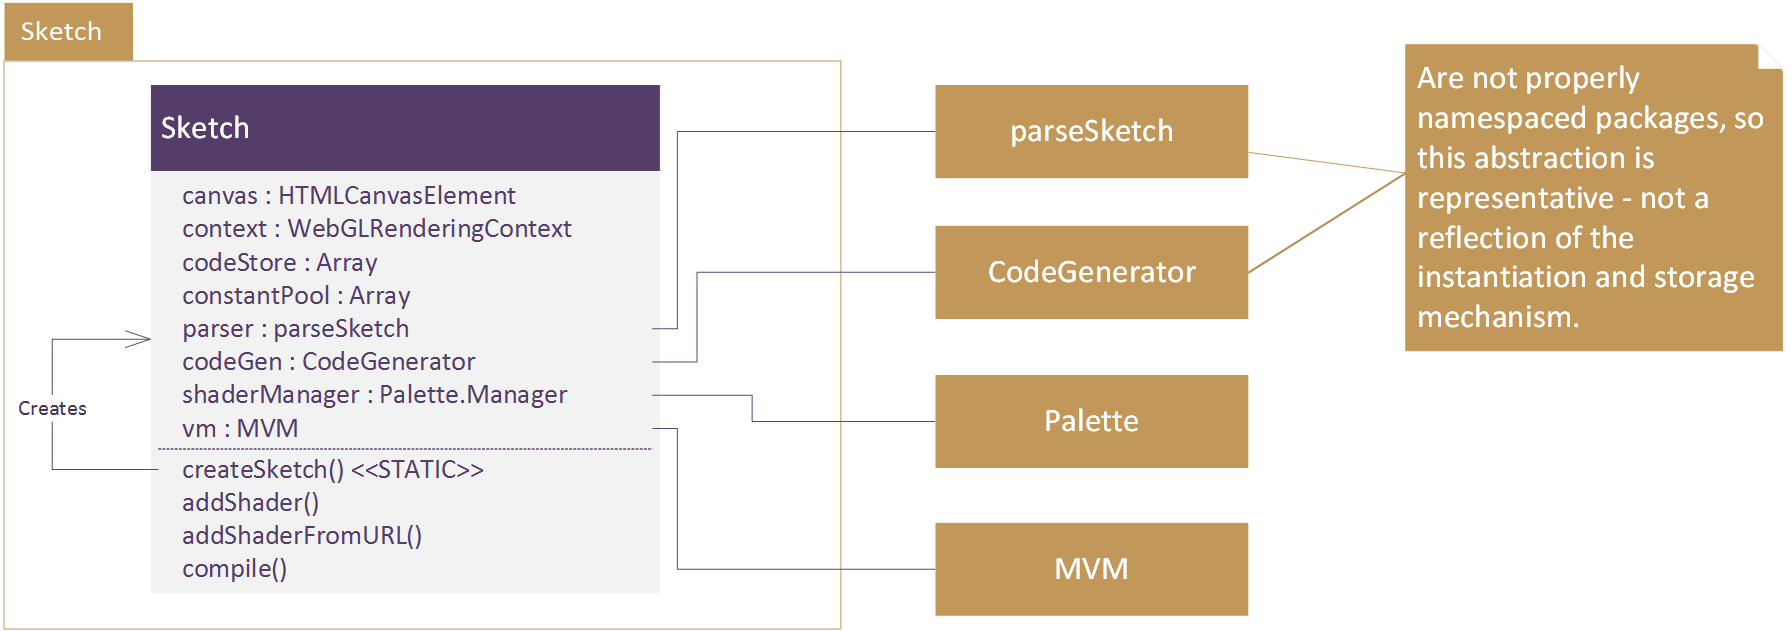
\includegraphics[width=\textwidth]{images/Facade-UML}
\caption{A UML class diagram of Sketch's module.}
\label{fig:module-uml}
\end{figure}

A fa\c{c}ade as shown in Figure \ref{fig:module-uml} was a necessity if we wished to provide users with the simple set-up we had envisaged. Although this component introduces no novel concepts, programming it still required the input of all team members to ensure that data would be properly handled between components.
\subsection{Implementation Process}
\label{arch-module-impl}
The implementation of the module provides very little functionality of its own, and merely abstracts the calls it receives to its registered components. From the beginning, we established that users would only desire to create an instance of the module, to add shaders to the system and to compile and execute Sketch source files they had written.

The only interactions which require functional code are adding shaders from URL, which delegates to the addShader method regardless, and program compilation. Program compilation follows the same execution order outlined in Chapter \ref{arch-over}, and executes the virtual machine as its final command. Aside from this, it must mediate between the components' output formats and the input arguments of the next step. For instance, the parser outputs the JSON string format of an object, which is functionally useless if we wish to traverse the tree in this form. This required communication between all team members who had developed components, to understand the data transformations required.
%==============================================================================
\chapter{Development Environment}
\label{dev}
For a project of this scale, distributed management of our development environment from the beginning was an absolute necessity. To keep source code management, building and recovery a simple process our system integrator devised a relatively robust system for the team to develop within.
\section{Source Management and Revision Control}
\label{dev-scm}
At the beginning of this year, most of our team were inexperienced with regards to proper source control systems - their operation differences, their configuration and their usage. Luckily, this meant that none of us would have to unlearn any SCM operation habits (as such platforms are notoriously different), and reduced the selection of a revision control system to one of availability and popularity. Our choices were narrowed down to two systems - \textit{SVN} and \textit{Git}.

From here, we decided that Git would be the ideal choice for our project's needs as it provides simple branch management, ease of access thanks to the rise of GitHub and an effective GUI client. Although some of Git's concepts were lost upon the team at first, we've since grown to be relatively adept at its operation. We've found it to be a great source of our effectiveness by enabling distributed collaboration for very little effort.

\section{Development Tools}
\label{dev-tools}
As our project is JavaScript based, there have been no provisions for an IDE or editor of choice - each team member used whatever they felt most comfortable with. Among our team Sublime Text was a popular choice as a pure text editor, with WebStorm occasionally being used by those who preferred a full IDE. All testing and code operation was performed within the browser as required by JavaScript.

\section{Build Management}
\label{dev-build}
The project uses Gulp (http://gulpjs.com/) for its build management solution. Gulp is a stream-based build system based around the automation of tasks - providing functionality such as concatenation, minification and documentation generation. Gulp is similar to Apache Ant and Maven, but eschews their configuration-driven approach in favour of a code-driven approach. We found this to be ideal, as it allowed the team to spend time working on their components with the build generation doing a lot of the menial tasks.

One particular strength was the litany of plugins available for Gulp - we found that we could automate our documentation production, library downloading and even the generation of our parser from its Jison file. Generation of these tasks was easy for the system integrator, and so the addition of new build tasks never added significant workload (unlike our past experiences with Ant and Ivy). Gulp is also the key to allowing us to provide a single JavaScript file for import by users, simplifying end-user implementation cost for Sketch greatly.

\section{Continuous Integration and Quality Metrics}
\label{dev-ci}
By choosing GitHub as our source control location, we allowed ourselves access to many continuous integration and code quality metric services - several of which are dedicated to providing free usage to open source projects. We decided to pursue Travis-CI (https://travis-ci.org/) as our CI framework of choice for several reasons. The primary consideration was the free cost for open source projects, a very important element in our decision process, followed by its built-in support for node.js based projects - ensuring that we'd be able to run Gulp builds without any hassle. We also anticipated adding a formal testing harness to the project, for which Travis would email the project administrator in case of failing builds, but found that this would be too much trouble and opted to stay with our collection of Sketch language test files.

Selection of a quality metrics service went through a similar thought process, leading us to CodeClimate (https://codeclimate.com/). We added this to our project as it had zero set-up cost (in both time and money) and provides a fantastic visualisation of code quality throughout the repository. While it often was passed over by the team, some members made great use of it by being able to quickly track down overly complex code, duplications and messiness in source files and fix code smells before they led to greater mistakes down the line.
%==============================================================================
\chapter{Online IDE}
\label{ide}
As part of our overall project plan, we decided that an environment for users to play around with Sketch was an essential deliverable for us to provide - both for our own testing purposes and to offer an interactive sandbox that could show off our project's capabilities.

\section{Design Process}
\label{ide-design}
Our team had not originally considered the production of a development environment for our language, until the topic had been raised by our supervisor in the language development stages. Up until that point we had merely assumed that users would produce programs on a desktop computer in their text editor of choice, before linking the code up to the module on a web-page via the JavaScript API. However, mobile devices were left with no means to write their own Sketch programs - this left out a potential user base that we were specifically trying to target by electing to use WebGL.

\begin{figure}
\centering
\begin{subfigure}[b]{0.45\textwidth}
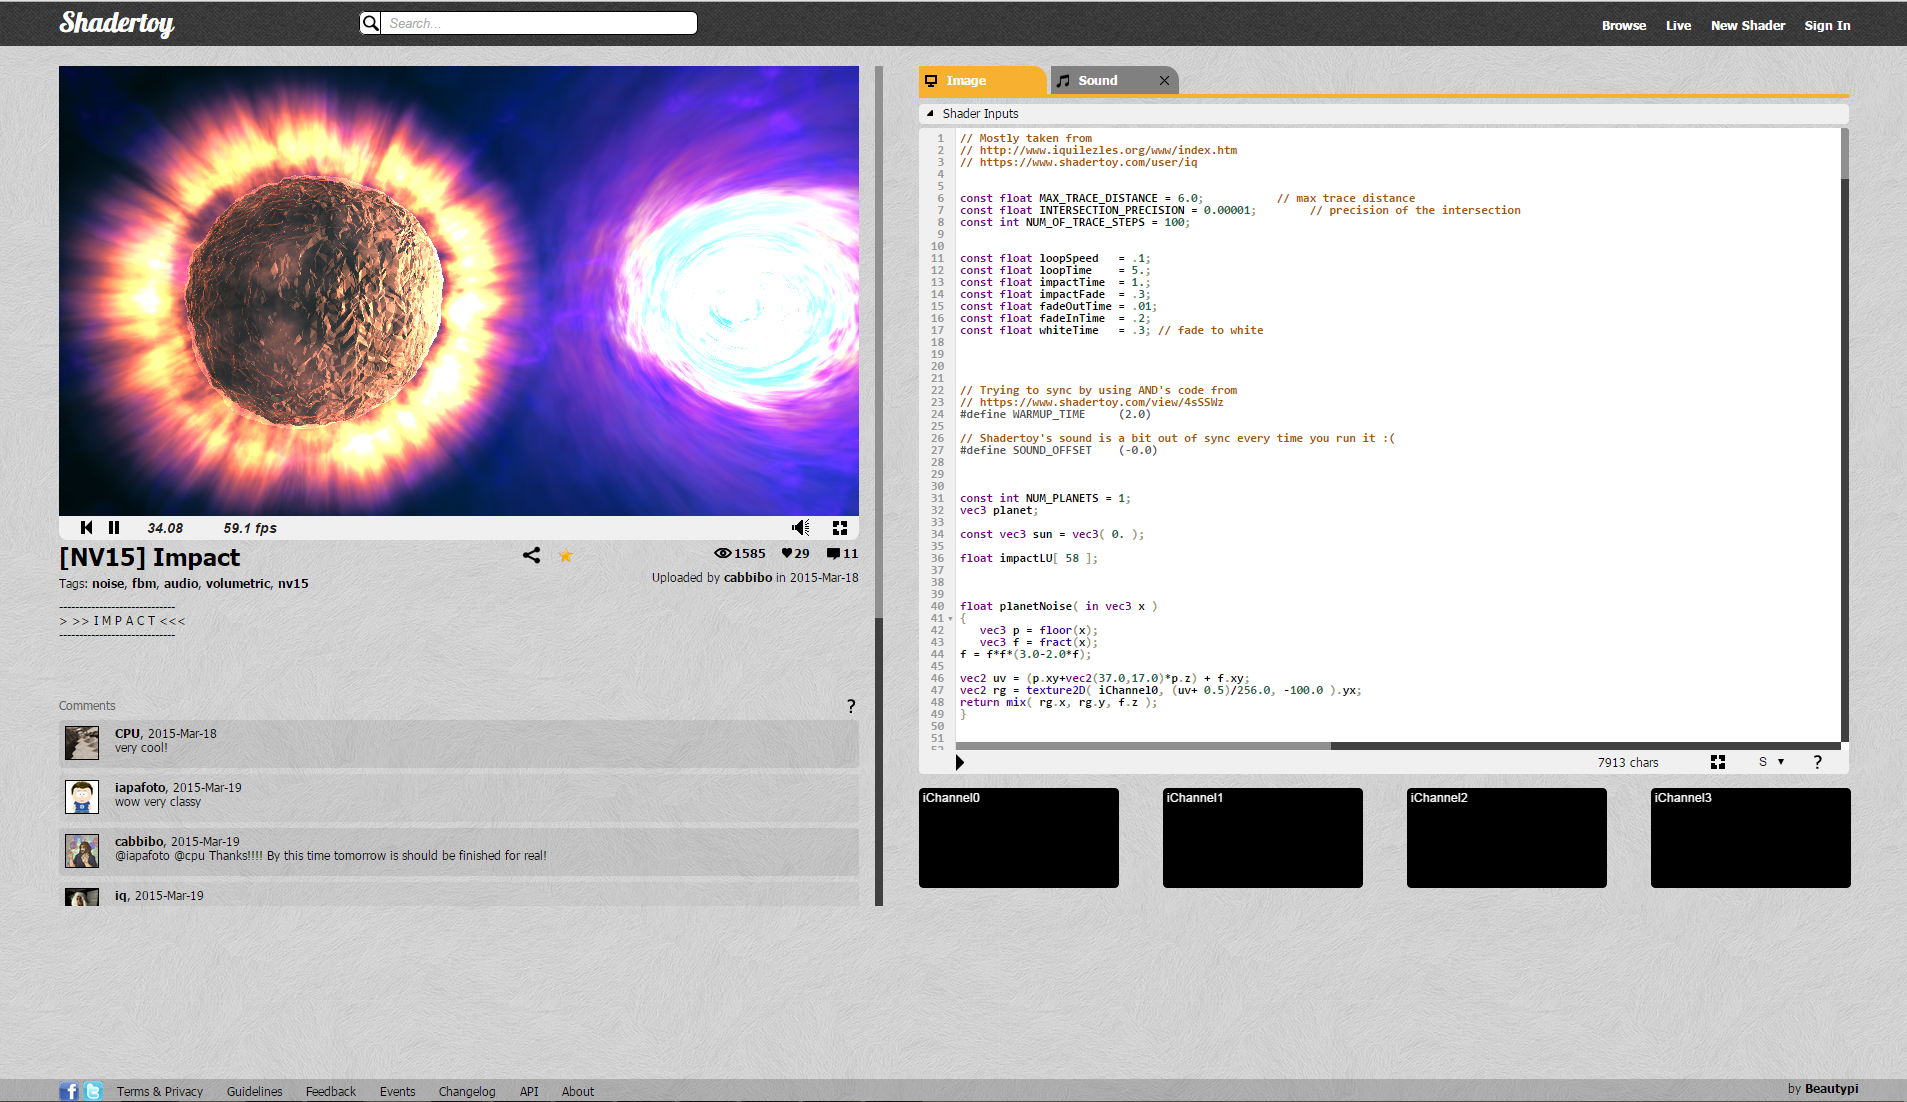
\includegraphics[width=\textwidth]{images/shadertoy-ide}
\caption{An image of ShaderToy's design layout.}
\label{fig:ide-shadertoy}
\end{subfigure}
\begin{subfigure}[b]{0.45\textwidth}
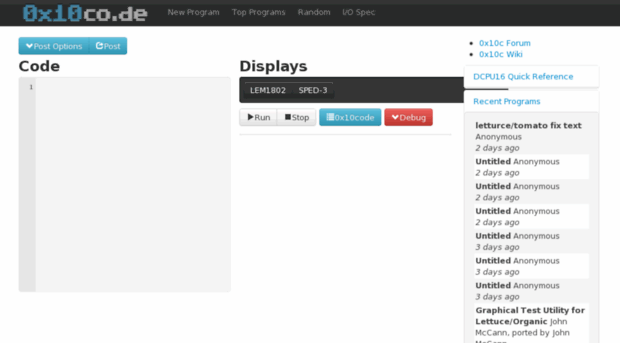
\includegraphics[width=\textwidth]{images/0x10code}
\caption{An image of 0x10co.de's design layout.}
\label{fig:ide-0x10code}
\end{subfigure}
\caption{Other online examples.}
\label{fig-ide-other}
\end{figure}

We began to look at existent online IDEs for various languages to serve as design inspiration for our own. Chief among these was ShaderToy (Figure \ref{fig:ide-shadertoy}), an online community built around sharing and discussing complex fragment shaders. ShaderToy's design makes the code and the visual output the primary focus for users, with both sections taking up relatively equal screen space at opposite ends of the screen. It's noted that the code segment takes up slightly more screen space - this is likely due to the far larger size of GLSL fragment shader code. While many elements of its design are bland, we found the structure of the page to be a perfect fit for graphics dependent languages where the canvas takes centre stage. We even found that the bland colour scheme of the site likely helped the key visual elements - the canvas and the code - to stand out to users by reducing visual clutter and noise elsewhere.\\

The now defunct 0x10co.de (Figure \ref{fig:ide-0x10code}), an online community based around the fictional DCPU-16, was another key influence in this regard - it also followed a minimalistic design scheme, placing code and graphical output at the forefront. We decided upon minimalism as our go-to style after our investigation to give the page and language presentation the purity we desired, and chose to go for a 50-50 split as our programs are intended to be relatively small. The key decision to deviate from the light pages in our two exemplars was made in light of modern trends within text editors such as Sublime Text - developers were regularly finding darker environments to be more aesthetically pleasing and less likely to cause eye-strain. As such, we decided to go for a darker web design; not only for these reasons, but also to enhance the appearance of the canvas by creating a stronger contrast.

\section{Implementation}
\label{ide-impl}
\begin{wrapfigure}{r}{0.4\textwidth}
  \centering
  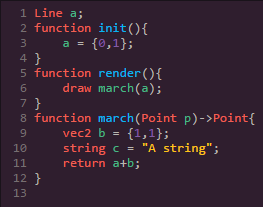
\includegraphics[width=0.38\textwidth]{images/sketch-syntax}
  \caption{Sketch's syntax colouring, provided by CodeMirror.}
  \label{fig:ide-syntax}
\end{wrapfigure}
On further research, it was noted that 0x10co.de and ShaderToy shared a common library - CodeMirror. CodeMirror is a JavaScript library designed to allow embedding fully formattable text entry boxes into web pages, with support for syntax highlighting, theme selection, various plugins and more. After researching it briefly, we were certain we'd found the right tool for the job.

Creating a new syntax colouration template was at first a difficult task - in essence, it was identical to building a parser for Sketch. Luckily, CodeMirror provides a simple module definition plugin, which reduces the task down to the construction of a finite state machine with the help of regular expressions. The task was far easier to tackle this way, and although it lacks the fine-grained control of writing a custom parser the results are very convincing. An image showing this colouring in action is reproduced for Figure \ref{fig:ide-syntax}. The state machine is as follows:
\lstset{%
      basicstyle=\ttfamily\footnotesize\bfseries,
      xleftmargin=.05\textwidth, xrightmargin=.05\textwidth,
      captionpos=b,
      tabsize=4
    }
\begin{lstlisting}[caption={Syntax Highlighting State Machine},label={lst:ide-fsm},language=JavaScript]
CodeMirror.defineSimpleMode("mlang",{
    start:[
        {regex: /"(?:[^\\]|\\.)*?"/, token: "string"},
		{regex: /(function)(\s+)([a-z$][\w$]*)/,
			token: ["keyword", null, "variable-2"]},
		{regex: /#.*/, token: "comment"},
		{regex: /\/\/.*/, token:"comment"},
		{regex: /true|false/, token: "atom"},
		{regex: /0x[a-f\d]+|[-+]?(?:\.\d+|\d+\.?\d*)(?:e[-+]?\d+)?/i,
			token: "number"},
		{regex: /\/(?:[^\\]|\\.)*?\//, token: "variable"},
		{regex: /\b(?:function|return|if|for|while|else|do
				|this|draw|clear|width|height)\b/, token: "keyword"},
		{regex: /\b(?:int|float|bool|string|Line|Point|Polygon|void
				|color|vec2|vec3|vec4|Circle)\b/, token: "keyword"},
		{regex: /\b(?:vector\([234]\))\b/, token: "keyword"},
		{regex: /[-+\/*=<>!]+/, token: "operator"},
		{regex: /[a-z$][\w$]*/, token: "variable"},
		{regex: /([a-z$][\w$]*)(?=(\s*)\()/, token:"keyword"}
    ],
    comment:[

    ],
    meta: {
        dontIndentStates: ["comment"],
        lineComment: "//"
    }
});
\end{lstlisting}

The page itself (Figure \ref{fig:ide-full}) is a very simple arrangement of blocks, a canvas, and a text area which is in turn replaced by CodeMirror. This is then styled by page-wide CSS designed to match our chosen CodeMirror theme - creating the subdued look we were going for.

\begin{figure}[!h]
\centering
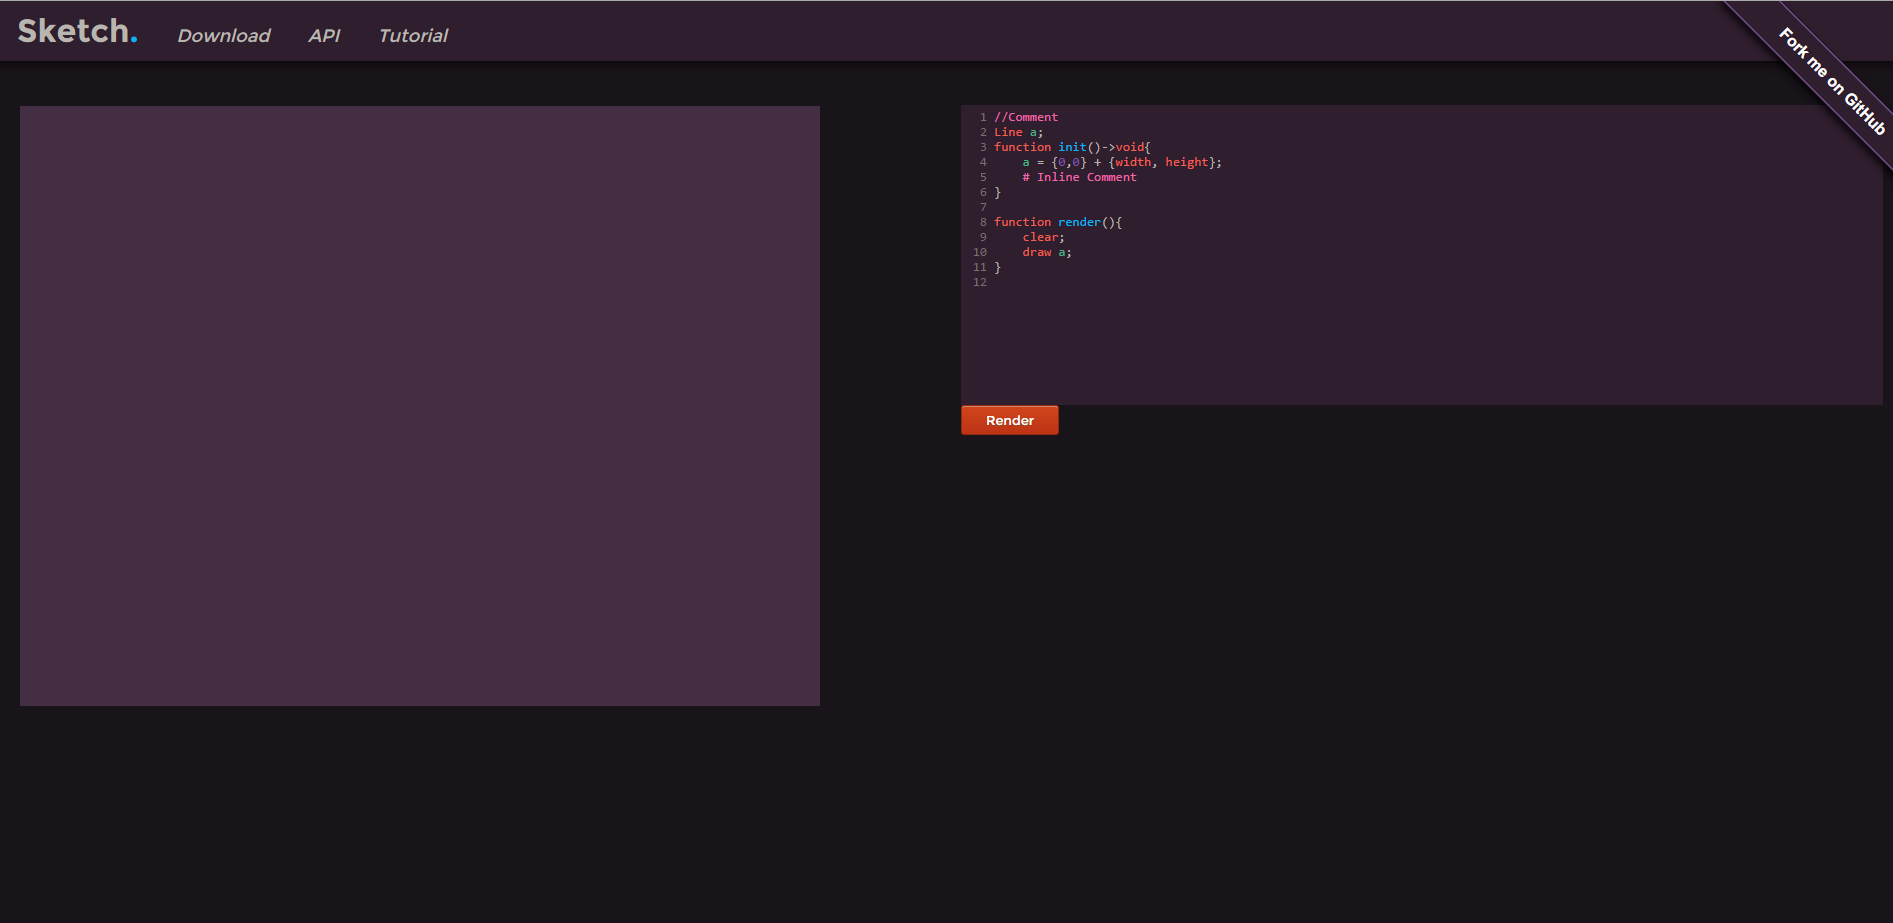
\includegraphics[width=\textwidth]{images/sketch-ide}
\caption{An image of the Sketch online IDE.}
\label{fig:ide-full}
\end{figure}
\section{Evaluation}
\label{ide-eval}
Being able to produce this page in less than two days, we realised that we had definitely made the correct choice in our library research. The page itself has much room to improve, however - there are vast amounts of unused whitespace, currently links to our documentation are non-functional and the page feels very barren, overall. We believe that the value that this aspect of our project provides is far greater than the time cost involved in creating it, thanks to the simple set-up process and the past experience of team members with HTML and CSS as well as its own intrinsic value.
%==============================================================================
\chapter{Test Plan and test suites}
\label{test}

%==============================================================================
\chapter{Conclusion}
\label{conc}

%------------------------------------------------------------------------------
\section{Contributions}
\label{cont}

%------------------------------------------------------------------------------
\subsection{Report}
\label{cont-report}

\textit{\textbf{Writing:}}
\begin{itemize}
\item \emph{David Creigh:} Chapter
\item \emph{Kristiyan Dimitrov:} Chapter \ref{arch-lex}
\item \emph{Gerard Docherty:} Chapter 
\item \emph{Darren Findlay:} Chapter 
\item \emph{Kyle Simpson:} Chapter \ref{arch-over}, \ref{arch-shad}, \ref{arch-module}, \ref{dev}, \ref{ide}
\end{itemize}
\textit{\textbf{Editing:}}
\begin{itemize}
\item \emph{David Creigh:} Chapter 
\item \emph{Kristiyan Dimitrov:} Chapter 
\item \emph{Gerard Docherty:} Chapter 
\item \emph{Darren Findlay:} Chapter 
\item \emph{Kyle Simpson:} Chapter \ref{tut}
\end{itemize}
%------------------------------------------------------------------------------
\subsection{Program}
\label{cont-prog}

%==============================================================================
\appendix
\chapter{Appendix A: Source Listing}
\label{appa}

Includes full source listing of compiler

%==============================================================================
\bibliographystyle{plain}
\bibliography{example}
\end{document}
